\section{Enabling Practical Multi-Acceleration} \label{sec:multi-acc}

\subsection{Motivation}
Accelerators are designed to provide fundamentally different energy-efficiency
and performance tradeoffs, depending on the properties of the application.
Actually achieving the potential speedup of multi-acceleration
requires practical techniques which can select the correct accelerator 
for the appropriate region of code.  The current research thus far,
outlined in Figure~\ref{fig:multi-acc-overview}, 
has only addressed the scheduling problem across uniform-ISA 
core types~\cite{Navada:2013:UVN:2523721.2523743,Lukefahr:2012:CCP:2457472.2457508},
which can only achieve modest efficiency gains.  These techniques are not
directly applicable to accelerators, as their tradeoffs are more distinct,
and their limitations are more restrictive. 


\begin{figure}
  \begin{center}
    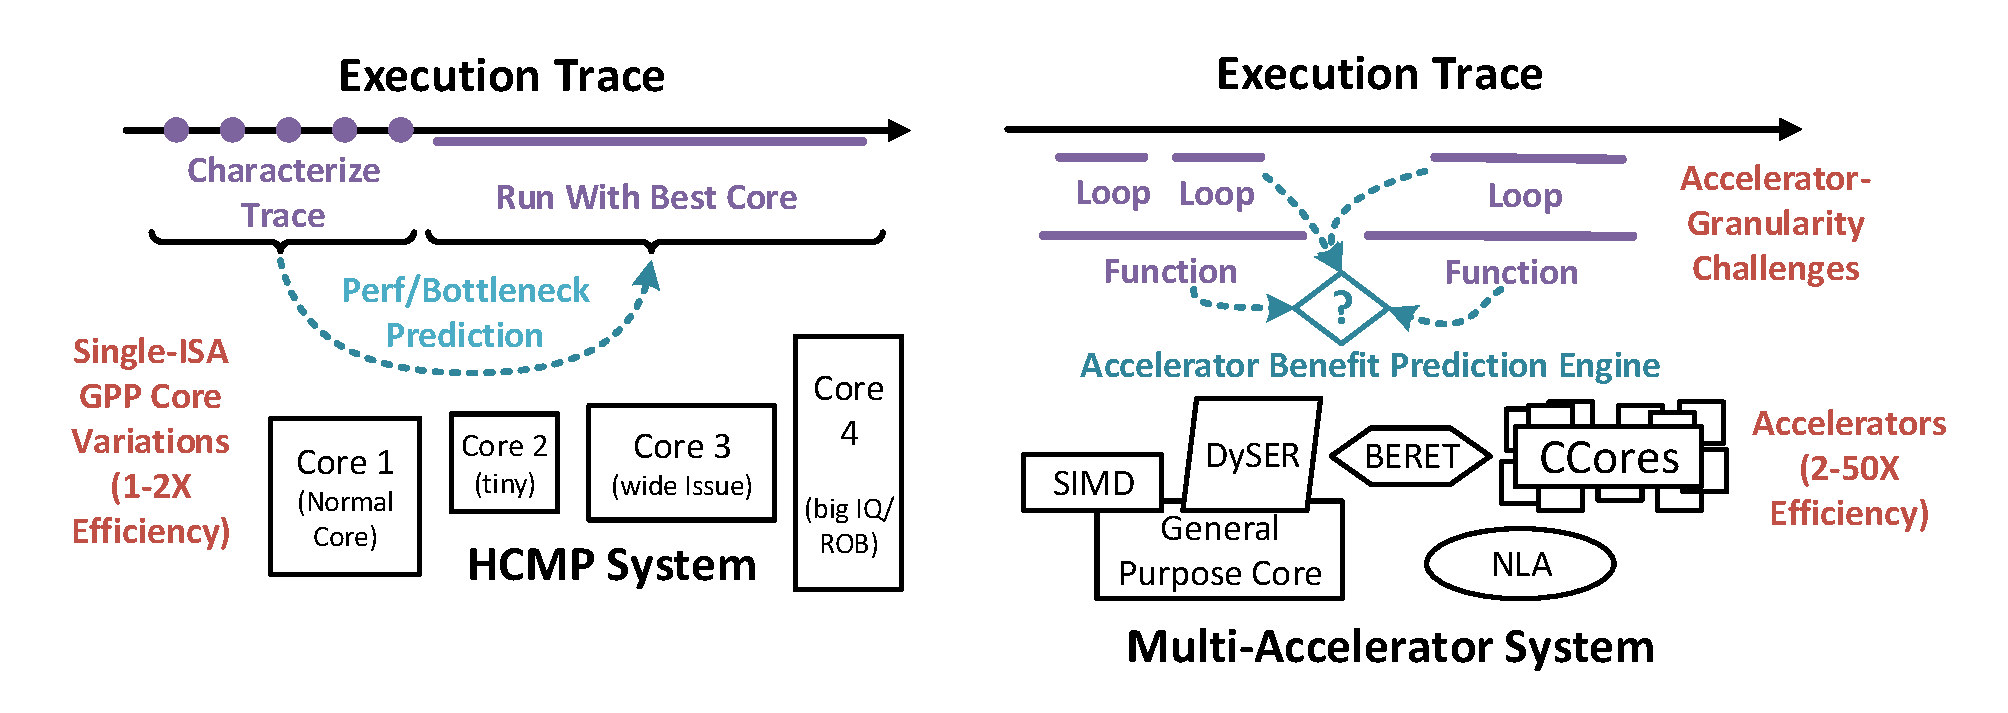
\includegraphics[width=0.8\linewidth]{figs/multi-acc-overview.pdf}
  \end{center}
\vspace{-0.2in}
  \caption{Current versus proposed approach for Multi-Accelerator scheduling.}
  \label{fig:multi-acc-overview}
\vspace{-0.05in}
\end{figure}


 
% Although in some cases the appropriate 
%accelerator may be intuitive, complex tradeoffs exist between acceleration
%strategies.  For example, should a control heavy code with loop independence
%target SIMD, or would it be better to utilize the custom datapath of a 
%Conservation Core.  Scheduling in a multi-accelerator setting inherently imposes 
%a variety of challenges, of which we enumerate next.

\begin{enumerate}

\item \textbf{Static versus Dynamic:} The first challenge is in whether the
accelerator scheduling should be static or dynamic.  More specifically, should a
compilation-time pass decide which regions should be mapped to which
accelerators, or should a runtime phase somehow profile the dynamic execution
and make decisions based on that.  Static algorithms can have a much higher
runtime, but dynamic approaches can take advantage of additional information.
The correct answer to this question will depend on whether there is a significant 
advantage in dynamism over time given a particular scheduling region.
Also, dynamic approaches cannot be used to decide whether baked-in accelerators
like Conservation Cores should be built in the first place, where as static-schedulers
could.

\item \textbf{Granularity of Scheduling:} The second challenge is that different
accelerators operate on different granularities, and hence overlap in their
scheduling regions.  For example the BERET architecture only targets traces of
inner loops, while Conservation Cores targets entire functions containing
potentially many loops, or can also target just inner loops.  
Since the decision of one region affects the other,
greedy decisions can lead to sub-optimal solutions. 

\item \textbf{Evaluation Metrics:}
Both energy-efficiency and performance are important metrics depending on the
setting, which could even change over time for a given device.  For instance,
a phone may want to switch from optimizing for performance to energy when
the battery is low.  Techniques which can provide flexibility would be ideal.

\item \textbf{Harmfulness of an Incorrect Decision:} Finally, in choosing a
certain accelerator for program region, an ideal solution would guarantee that
at a minimum, whatever performance or energy-efficiency is provided by the
general purpose processor is preserved by the accelerator.  However, it is
possible that accelerators can degrade either metric.  Care must be
taken not to do more harm than good.

\end{enumerate}

\subsection{Research Approach} Before designing techniques for enabling
multi-acceleration, we first explore whether there is inherent value.  Also, as
it is an unexplored topic, the way forward in integrated, automatic 
multi-accelerator scheduling is
unclear.  Therefore, it is prudent to develop and compare a variety of
strategies which have different tradeoffs.  The remainder of this section
describes four initial approaches which will be investiaged, and also describes
a mechanism for handling multi-granularity which is common across techniques.

\paragraph{Value of Multi-Acceleration}  
Results from section~\ref{sec:limits} provided quantitative evidence
suggesting there exists significant energy-efficiency and performance 
benefit from utilizing different accelerators on different benchmarks.
Going further, Figure~\ref{fig:benefit-multiacc} shows the benefits of
multi-acceleration for both the inorder and OOO core.  On the bottom half of
each graph is the percentage of time each accelerator is the most beneficial
in terms of performance.  There are several useful observations here, first,
structured hardware accelerators like Conservation Cores and BERET are much
more utilized on the inorder core.  More importantly, even within a single
application, depending on the region being accelerated, different regions
favor different accelerators, some even using all five(including
no-accelerator) design points.  On the top half of the graph is amount that
each benchmark is sped up over choosing just one accelerator for that
benchmark.  For some benchmarks, multi-acceleration at a fine granularity can
have up to 50\% performance improvement.  We expect these numbers only
to increase with further accelerator development.

\begin{figure}
\begin{adjustwidth}{-0.75in}{-0.75in}
\begin{center}
\footnotesize
\def\arraystretch{0.25}
\begin{tabular}{cc}
\textbf{Inorder Core} &
\textbf{OOO Core} \\ 
    \multicolumn{1}{ c }{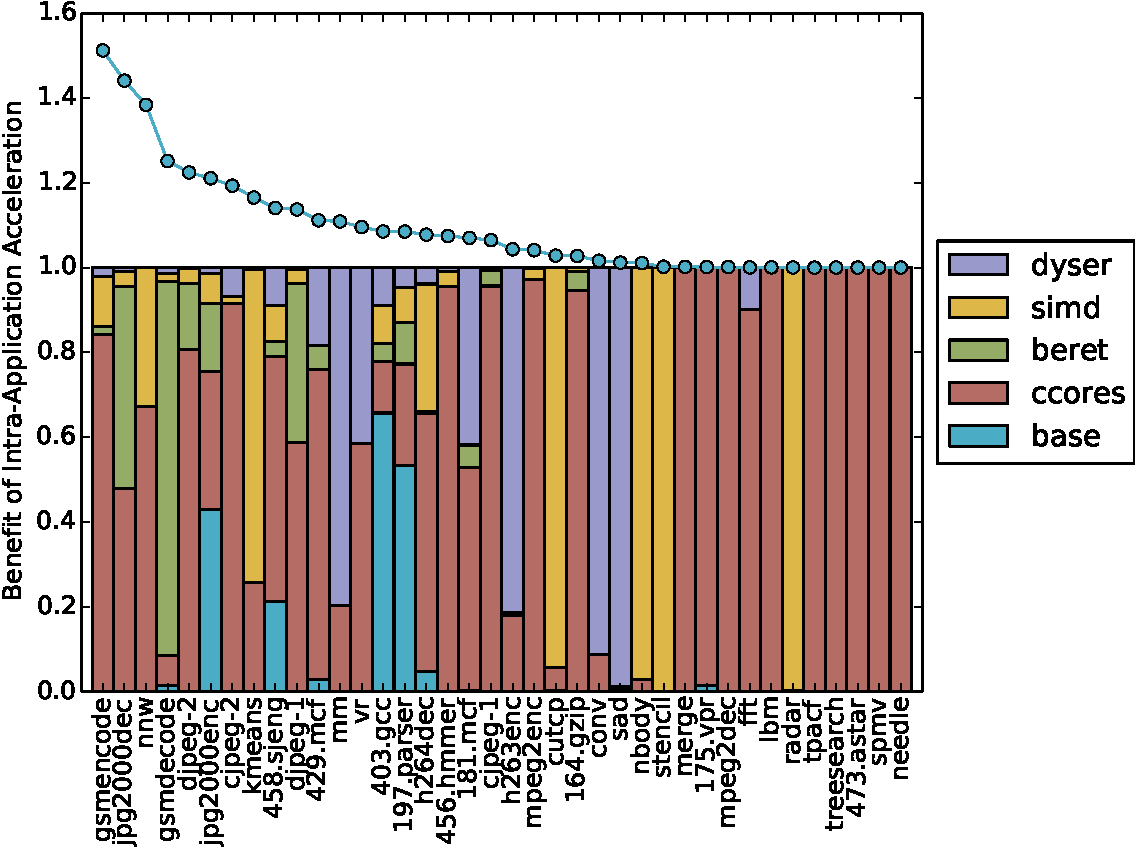
\includegraphics[
                         width=0.44\linewidth]{figs/multi_benefit_default_inorder.pdf}} &
    \multicolumn{1}{ c }{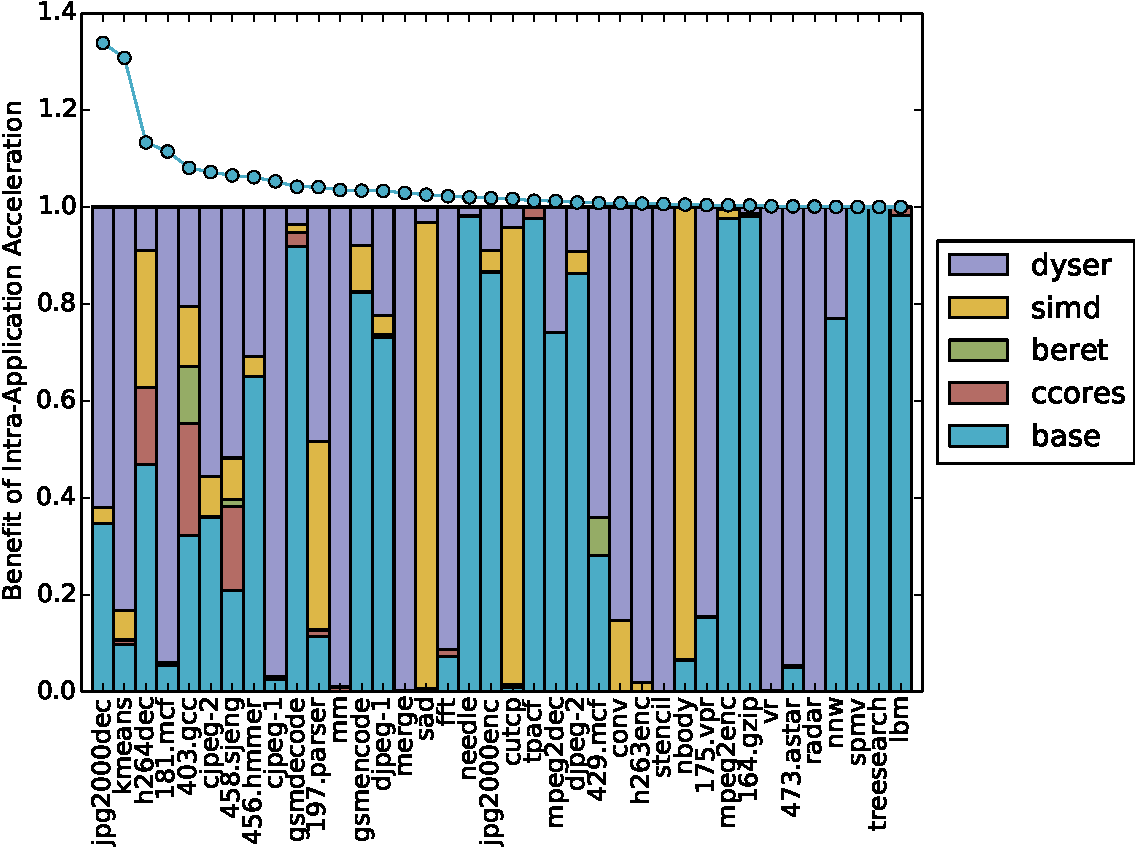
\includegraphics[
                         width=0.44\linewidth]{figs/multi_benefit_default_ooo.pdf}} \\
\end{tabular}
\end{center}
\vspace{-0.1in}
\caption{Benefits of Fine-Grain Multi-Accelerator Scheduling}

\label{fig:benefit-multiacc}
\end{adjustwidth}
\end{figure}

\paragraph{Program Structure Tree}  As mentioned earlier, scheduling is made
difficult because the choice to schedule at one granularity could preclude a
beneficial scheduling at a finer or coarser granularity.  This problem is
easily solvable using a greedy algorithm if we have perfect information of how
much benefit each accelerator provides at each scheduling granularity.  To do
this, we require a structure called the program structure tree (PST).  It is
highly related to the call graph, except that it also includes nodes for loops
and traces through loops that can be targeted by certain accelerators, and it
also doesn't naturally handle recursion.  This is acceptable for our use case
since none of the accelerators we model can utilize recursion.   

\begin{figure}
  \begin{center}
    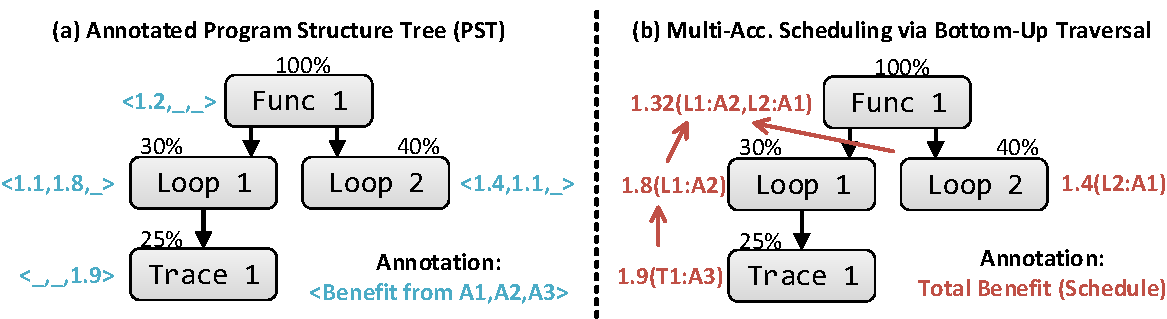
\includegraphics[width=\linewidth]{figs/pst.pdf}
  \end{center}
  \caption{Scheduling via the Program Structure Tree (PST)}
  \label{fig:pst}
\end{figure}

Scheduling can be performed on the PST as we describe next.
Figure~\ref{fig:pst}(a) shows an example PST which is annotated with the
percentage of execution time each region is responsible for, along with a
``benefit,'' vector, where each entry represents the amount of benefit each
accelerator can provide over the general purpose processor in terms of a
certain metric.  In this example we assume performance is the metric of
interest.  Figure~\ref{fig:pst}(b) shows how to traverse the tree from bottom
up to compute the schedule.  At each node in the tree, a decision needs to be
made whether an acceleration at the next lower level, or the current level is
better.  For performance calculation we can apply Ahmdal's law.
For example, ``Loop 1,'' must choose whether accelerating at ``Trace 1'' or at
it's own granularity is better.  Using Ahmdal's law, using ``Trace 1'' inside
Loop 1 would yield a speedup of: $1 / ( (1-\frac{.25}{.3})+.\frac{.25}{.3}/1.9)
= 1.65\times$ performance.  This is worse than the best acceleration at
granularity ``Loop 1,'' so ``Loop 1'' instead selects accelerator 2 (A2) at
it's own granularity.  This continues until the top of the tree, where all
scheduling decisions would be made.

Of course, attaining the information necessary for using this strategy is the
more challenging aspect of multi-granularity scheduling.  Below we describe
four techniques, the first uses an adhoc technique which does not require the
PST, and the other three techniques utilize the PST.


\paragraph{Static Technique: Intuition-Guided Scheduling} Perhaps the most straightforward
method of scheduling is to use heuristics to decide if a region should be
scheduled to a particular accelerator.  For example, if an inner loop has 
independent iterations, and the communication cost is low, the DySER architecture
might be the best choice.  Else, if the DySER communication cost is high, choose
SIMD.  This is the only scheduling technique we propose that does not use the PST
for scheduling, and as such, it can miss out on acceleration opportunities from
lack of multi-granular scheduling.

\paragraph{Static Technique: TDG-Based Prediction}
An alternate static approach would be to re-purpose the TDG as a prediction device.
Instead of generating a dependence graph from the binary trace as we do now, we could
build the graph for different accelerators based on the compiler's intermediate 
representation.  Of course, dynamic latencies (memory latency, misprediction latency),
and program inputs (to determine loop iteration/function counts) would have to be 
estimated, or Monte-Carlo (randomization) techniques could be employed. The predictions,
and estimated region time would be fed to a PST traversal for scheduling.

\paragraph{Dynamic Technique: Mixed-Granularity Sampling} The most natural dynamic
approach would be a sampling based one.  When the GPP reaches an acceleratable
region, it could try each legal accelerator for that region in turn for some
short number of cycles.  Sampling would have to occur at multiple
granularities, and calculating the best choice would entail a PST traversal at
run-time per scheduling decision.
After attaining samples and making a decision, it could run the best accelerator for some longer period of time before recalculating.  The primary overhead here is in 
the many samples which would be required for the PST traversal,
where many inopportune accelerators would have to be temporarily applied.

\paragraph{Dynamic Technique: Machine Learning} As other researchers have
discovered, the performance of an accelerator may be able to be predicted by
machine learning techniques which interpret properties of the general purpose
processor's execution.  One approach would be to use performance counters as an
input to a regression model to predict the metric of interest. Note that this
technique obviates the need to actually run on the accelerator prior to making
a decision, so should incur much less frequent switching and overall overhead.
However, the overhead of PST traversal would still be required.  Linear
regression is one viable candidate for a machine learning technique as it can
be computed extremely efficiently.  
 
%\textbf{Karu: Can I somehow mention that these ideas came from Newsha, or there is
%potential collaboration opportunities?  Or I can stay away from this idea if you prefer?}
\begin{figure}
\begin{center}
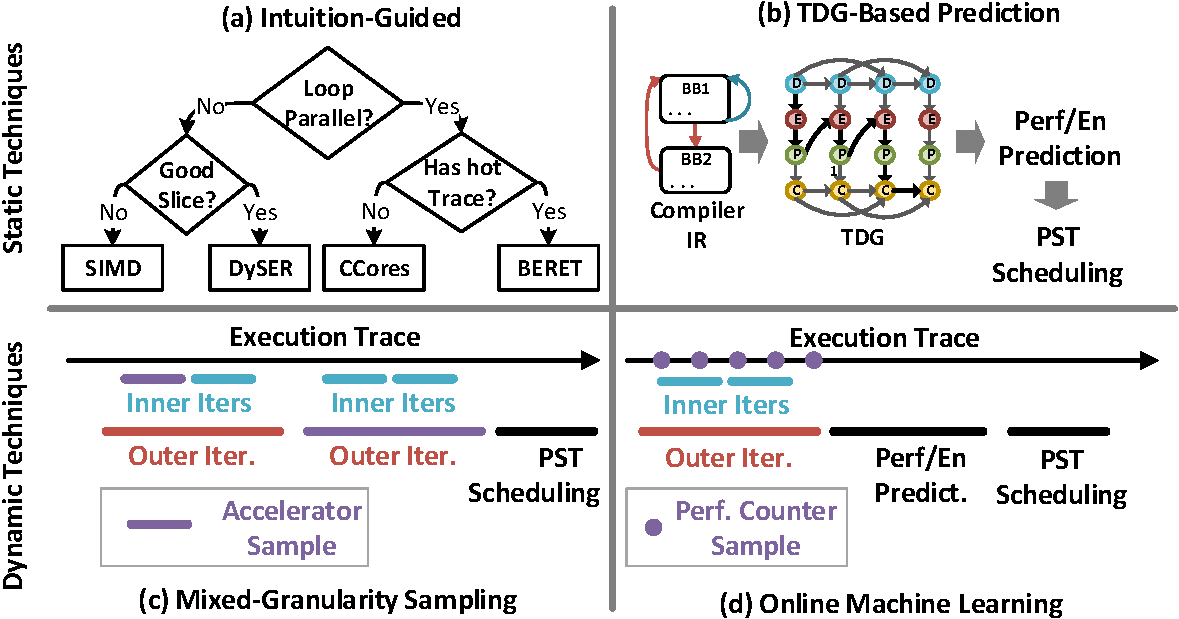
\includegraphics[width=0.84\linewidth]{figs/multi-sched-techniques.pdf}
\vspace{-0.05in}
\caption{Potential Scheduling Techniques}
\label{fig:sched-techniques}
\end{center}
\vspace{-0.1in}
\end{figure}

\if 0
\begin{figure}
\begin{adjustwidth}{-0in}{-0in}
\begin{center}
\footnotesize
\def\arraystretch{0.25}
\begin{tabular}{cc}
%   \multicolumn{2}{ c }{stuff}  \\ \toprule
%   \multicolumn{1}{ c }{\textbf{Performance}} & \multicolumn{1}{ r }{\textbf{Energy}}  \\ \toprule
%Performance & Energy \\ \toprule
\toprule
    \multicolumn{1}{ c }{(a) Intuition Based} &
    \multicolumn{1}{ c }{(b) TDG-Based} \\

    \multicolumn{1}{ c }{Fig Here} &
    \multicolumn{1}{ c }{Fig Here} \\

\midrule
    \multicolumn{1}{ c }{(c) Mixed-Granularity} &
    \multicolumn{1}{ c }{(d) Machine Learning} \\
%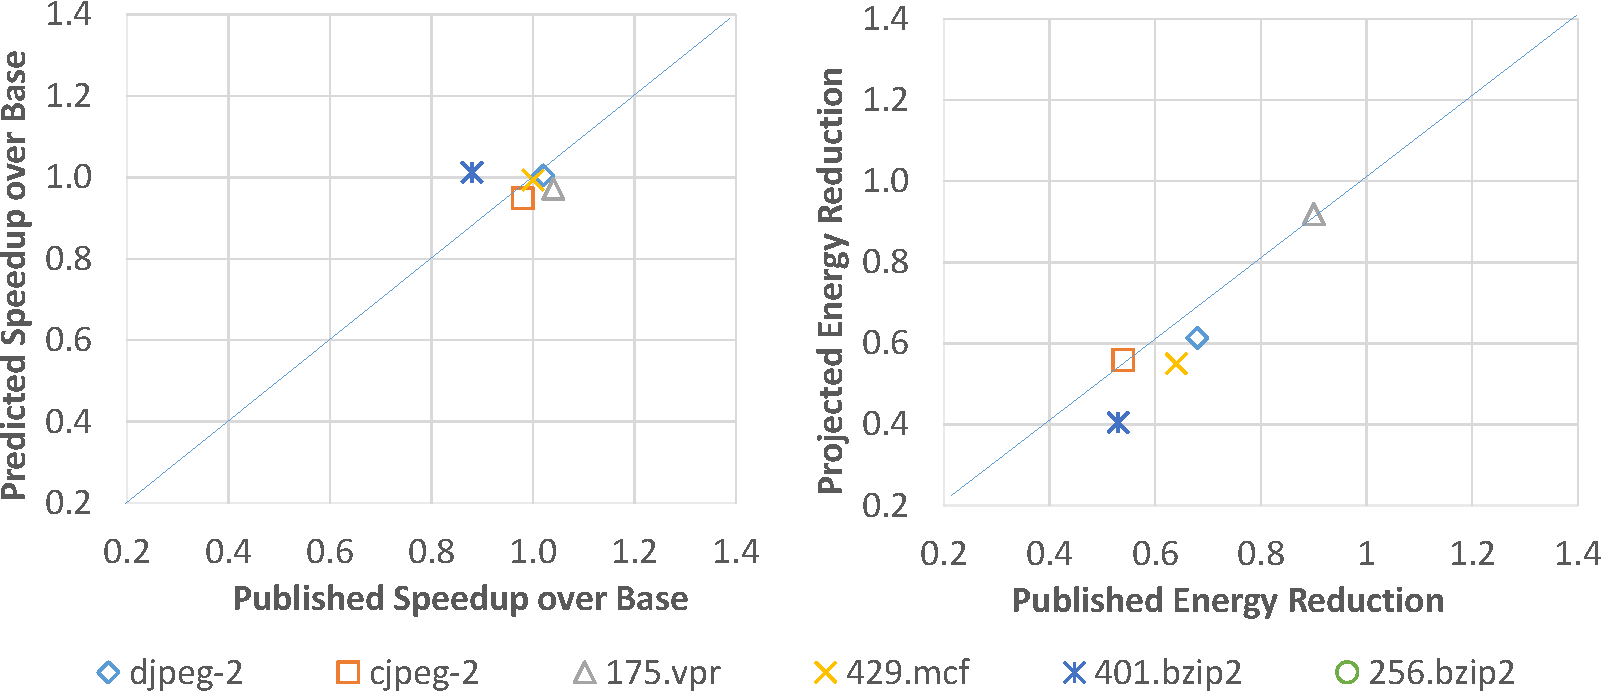
\includegraphics[width=0.44\linewidth]{figs/v_ccores.pdf}

    \multicolumn{1}{ c }{Fig Here} &
    \multicolumn{1}{ c }{Fig Here} \\
\bottomrule

\end{tabular}
\end{center}
\vspace{-0.1in}
\caption{Potential Scheduling Techniques}
\label{fig:sched-techniques}
\end{adjustwidth}
\end{figure}
\fi

\subsection{Proposed Work}

\paragraph{Static vs. Dynamic Scheduling Analysis}
We will first investigate whether we should
immediately rule out either static or dynamic scheduling.  We can do this by
determining the best dynamic schedule for a particular application by running
the application with the current set of models, and recording the cycles during
region transitions.  We can then compare the best acceleration where the
acceleration is always the same as one where we allow the accelerator to
change across instantiations of the region. 
 
\paragraph{Scheduler Implementations}
The next task is to create a version of the TDG which is multi-acceleratable.
Currently, only one acceleration transformation can be applied to an entire
program.  Further implementation will allow the graph to accelerate
different portions with different accelerators.  After this, depending on what we
decided about static/dynamic scheduling, we will implement the proposed scheduling
techniques.

\paragraph{Scheduler Evaluation}
For evaluation, we will target a variety of accelerator compositions, including
the most challenging composition which incorporates all accelerators considered
so far, even the nested loop accelerator (NLA) described in the previous section.
We will compare both how much raw benefit they can provide in
performance and energy efficiency, and also how flexible they are in targeting
different goals (speedup, energy efficiency, or some combination).  The larger
question we hope to answer is whether or not multi-acceleration is
practically achievable, and how much benefit is likely to come from it.

%\subsection{Preliminary Results} 
%
%\paragraph{Opportunities with No Limitations}
%Show best schedule for the program, versus the best schedule for each for each
%region, with no limit relaxations.
%
%\paragraph{Opportunities with Limits Relaxed}
%Show best schedule for the program, versus the best schedule for each for each
%region, with some limit relaxations.


\subsection{Related Work} Heterogeneous scheduling has been addressed before in
different settings.  One example is work which uses FabScalar to create
heterogeneous single-ISA multicore~\cite{Navada:2013:UVN:2523721.2523743}.
The technique they use is to treat one core as the baseline core, and switch
to ``accelerator'' cores to alleviate certain bottlenecks in applications.
While conceptually similar, this related work targets processors with only minor
relative performance benefits, does not deal with the mixed-granularity
problem, and does not face significant risk from incorrect choice.

Another example is Composite Cores, which uses two different frontend
pipeline designs to feed
the same back-end~\cite{Lukefahr:2012:CCP:2457472.2457508}.  One front end is
high-performance and out-of-order, while the other is in-order and
energy-efficient.  In their scheduling paper, they show how to use trace
based prediction mechanisms to out-predict simpler sampling
techniques~\cite{conf/micro/PadmanabhaLDM13}.  Our work differs substantially
because we are targeting accelerators that go far beyond merely
changing the microarchitecture for a ISA.  The proposed work targets
fundamentally distinct architectures which can provide
potentially an order of magnitude further energy-delay improvement.


